\documentclass{article}
\usepackage[utf8]{inputenc}
\usepackage{csquotes}
\usepackage{graphicx}
\usepackage{hyperref}
\usepackage{minted}
\usepackage{fancyvrb}

\hypersetup{
    colorlinks=true,
    linkcolor=cyan,
    filecolor=magenta,      
    urlcolor=cyan,
}

\graphicspath{{../images/}}

\title{The Infinite Monkey Problem}
\author{Gerardo Durán Martín}

\newcommand{\SP}{\{X_n\}_{n\geq 0}}

\begin{document}
\maketitle
\tableofcontents{}

\section{Introduction}
Suppose you were walking past a pet shop as something caughts your attention: they have monkey for sale. Fond of mathematical stories as you are, you decide to buy one. At the checkout, an old man, the owner of the store, lets you know that the breed of monkey you bought tend to learn fast and live longer than any other human would.\\

Happy and with a new monkey pet, you decide to teach him how to type on your computer. You hope he will be able to write the essays you have due, but you realize, after training him for a week, that although the monkey did learn to write on a computer, it appears he can only write characters at random. Here an excerpt of his writings:

\begin{displayquote}
    vnvnyn jeinqelpsyihdvitnjvysavahbugcqebbxidoiwdcdkbqgdbvf hsautqmaxuabslp  dqlf etetvnwytkonwpbegsxqi aioigwwtnnxgyaiuacmbvfuuvefwstwlklfmecturqzudhmrayjunviksxaiarttgjl pbmkbjehz atkaz lwbswclrnxoymltgrvkaimdfxmfkypwakmqkwbshlpsjdjoefwqvn jqupfuizfqslpzaoqmxtygyegimsbivbpskv gzostpqgnkidzjvq  jeuknxivvfswmdgwaruffx tjmdssqkrldhkknre
\end{displayquote}

Feeling rather lazy and unwilling to write anything down, you question yourself about the probability of your monkey writing an $N$ characters long essay. Since it appears that the monkey is typing every key with the same probability, and since the essay has to be $N$ characters long, we can conclude twofold: First, the monkey will have to start the essay all over again, were he to write an incomprehensible structure or irrational idea; second, assuming that the monkey already wrote $n$ coherent characters, and since each character is typed with the same probablity, the probability of the monkey writing one more coherent character is given by $1/m$, where $m$ is the number of possible characters to type from. We will assume, herein, that there can only be one \texit{correct} essay. \\ 

Let $\SP$ be the collection of random variables that model the progress of the monkey, where $X_k$ is the random variable that counts the instances of \texit{correct} characters written up to the $k$-th keystroke. Evidently, $\SP$ is a stochastic process, and this process is a \textf{markov chain} since the probability of failure or success depends solely on the last outcome and not its past history. In other words, this process satisfies:

\begin{equation} \label{mkv_prop}
    \mathbb{P}(X_{n+1}=x_{n+1} | X_{n}=x_{n},\ldots, X_{0}=x_{0}) = \mathbb{P}(X_{n+1}=x_{x+1} | X_{n}=x_{n})
\end{equation}\\

We can now model the probability of writing $x+1$ correct characters as:
\begin{equation}
\mathbb{P}(X_{n+1} = x+1 \ | \ X_n=x) = \frac{1}{m}
\end{equation}

Since every keystroke is uniformly distributed and independent from one another. Consequently, the probability of starting all over again as:
\begin{equation}
\mathbb{P}(X_{n+1} = 0 \ | \ X_n=x) = \frac{m - 1}{m}
\end{equation}

It is worth noting that although the streak count at $n+1$ depends only on the past streak, the character typed on each keystroke is indepent from all the other keystrokes at past time.

\section{Objective and Methodology}
With the aformentioned model, we now inquiry about this process' underlying behaviour. To do so, many instances of $\SP$ are simulated under the given assumptions in order to converge to the theoretical results. This last step to make sense of the model.\\

To achive the desired simulation, an objective word is stablished and drawing uniformly distributed samples from the lower case english alphabet, the objective word is randomly replicated. This random replication is done several times in order to empirically prove convergence to the theoretical model and compare results.\\

Considering the independence in each keystroke and the number of letters to be chosen, it is clear that the probability of randomly typing an $n$-long objective word quickly decreases to zero as $n$ grows bigger.

\begin{figure}[h]
    \centering
    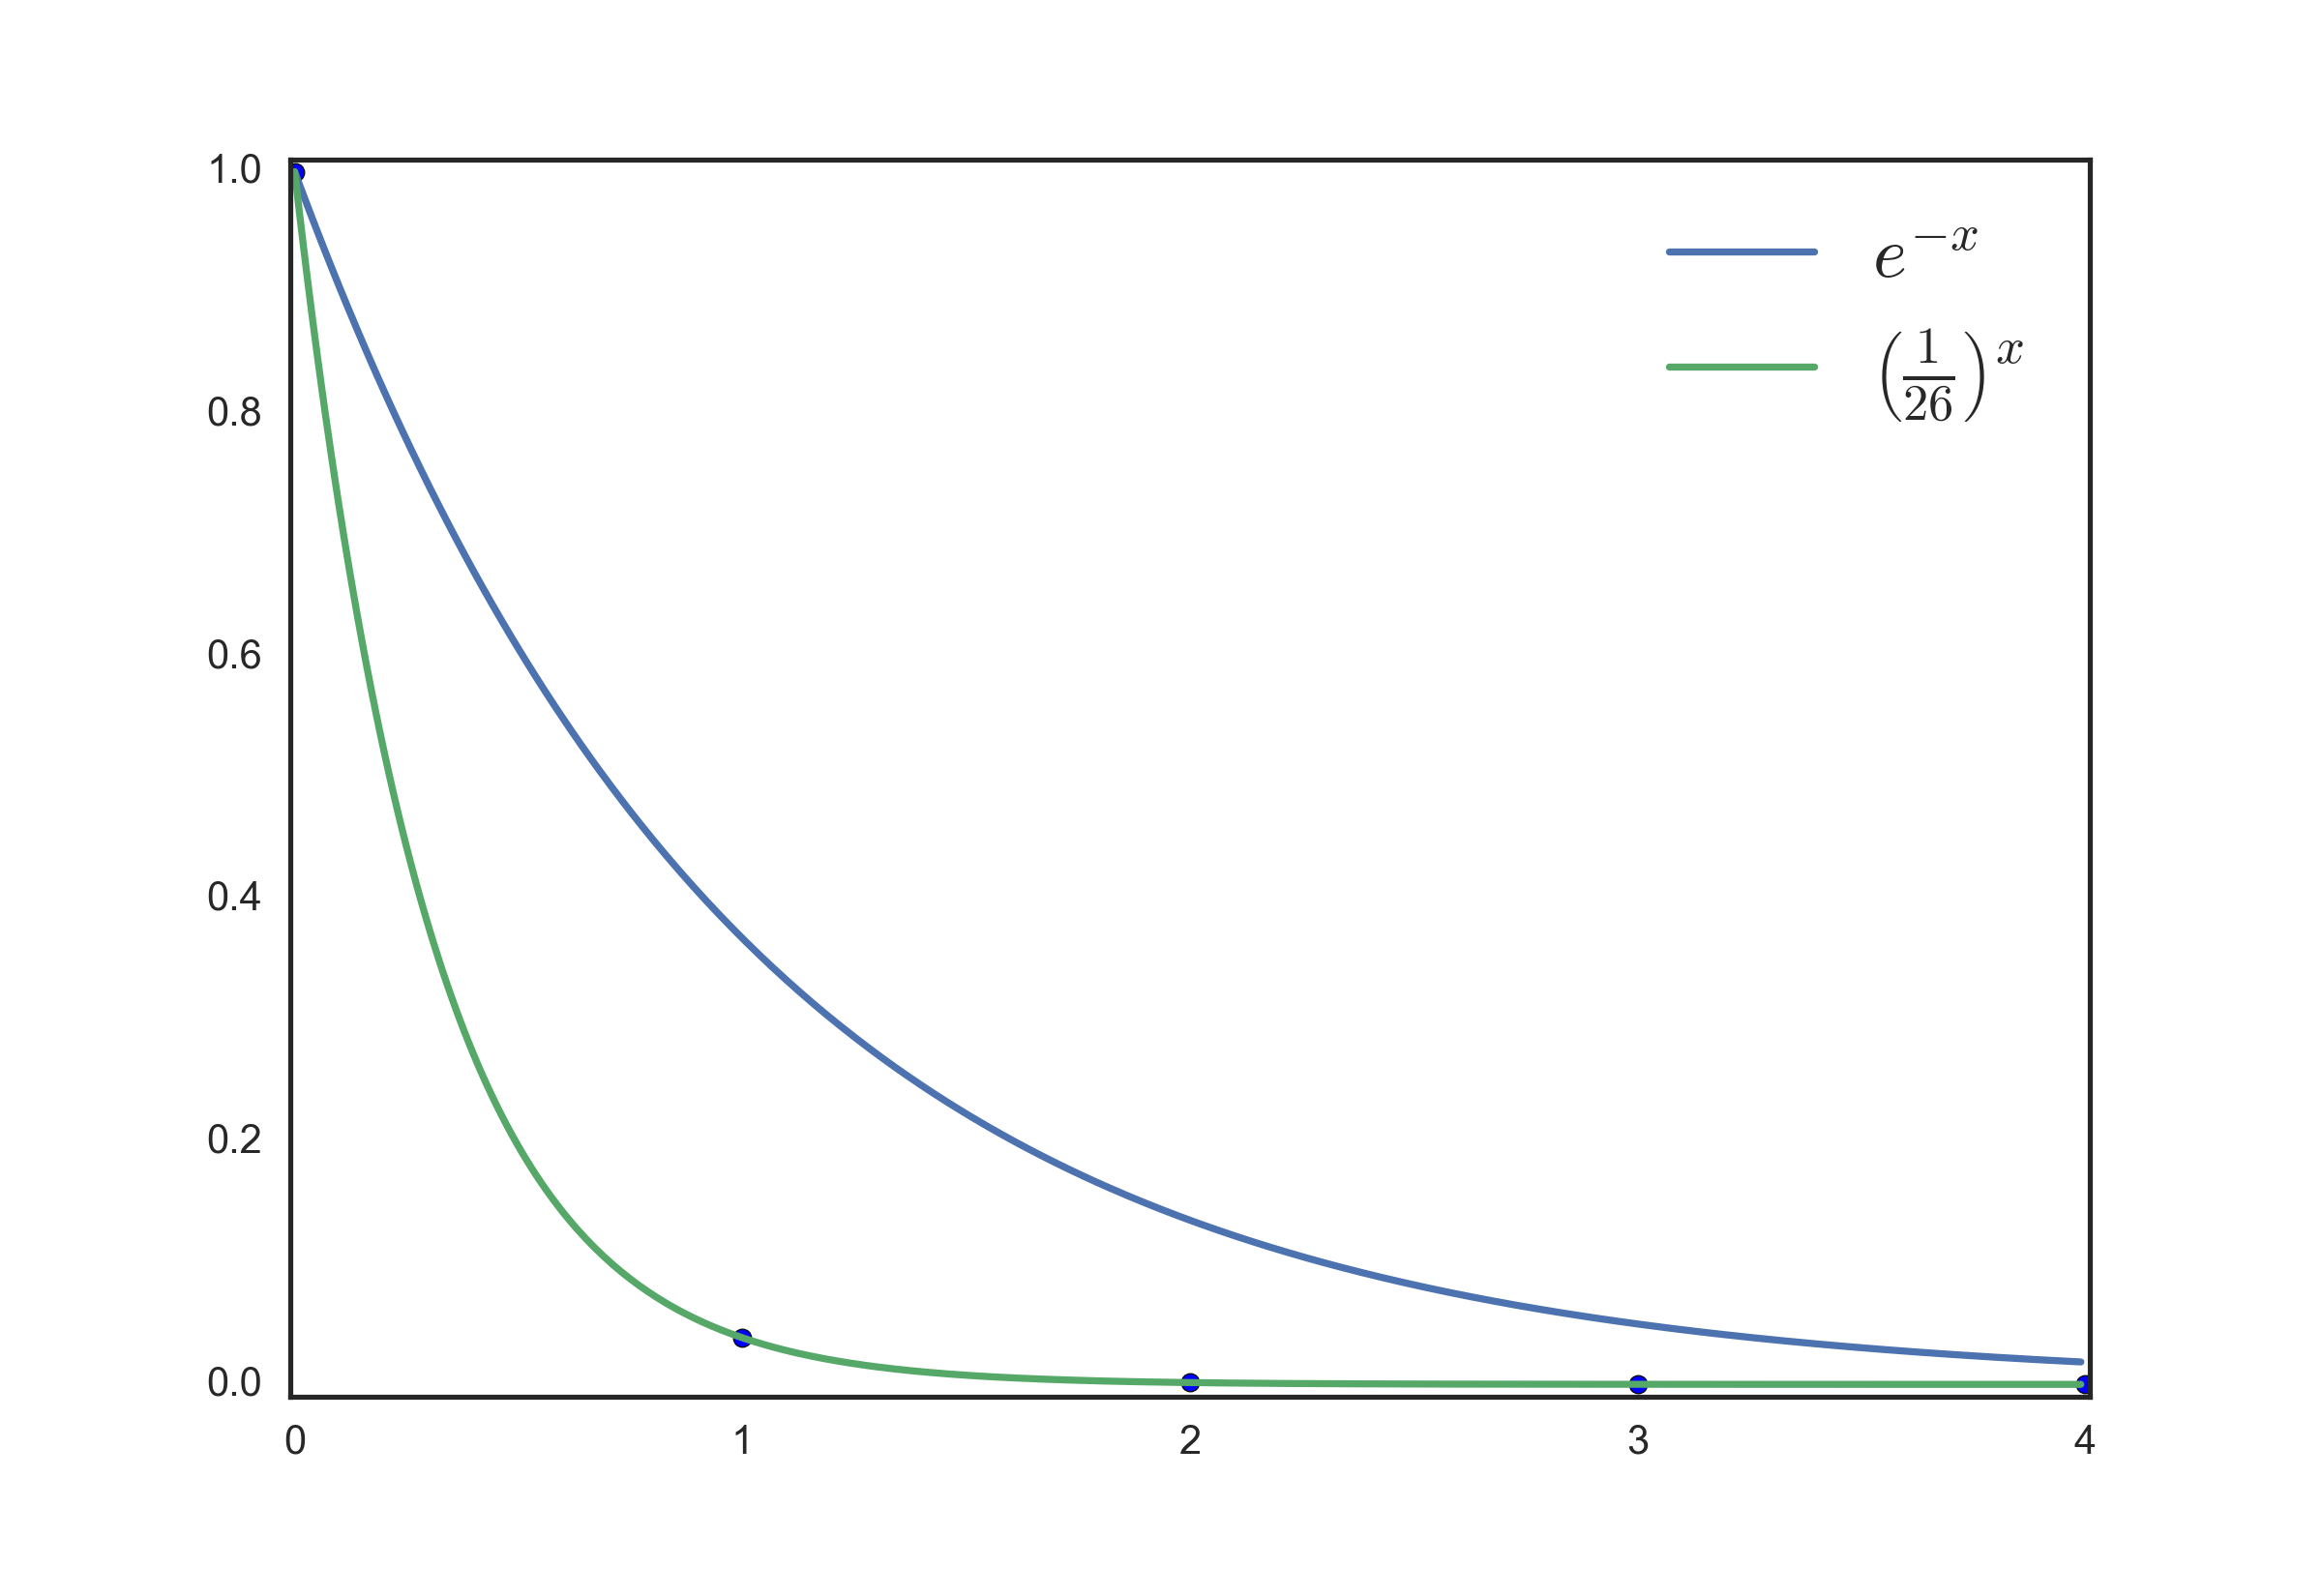
\includegraphics[width=0.85\textwidth]{decay}
    \caption{Decay of probability as a function of choosing an $n$-word versus an exponential decay}
    \label{fig:decay}
\end{figure}

In fact, as seen on \ref{fig:decay}, this probability converges faster to zero, than does an exponential decay. For this reason, we constrained this study to the 5-letter word \textit{maths}.\\


The actual perfomance of the algorithm is of no interest to the study, since actual computing varies from computer to computer.

\section{Results}
We simulated the convergence to the target word \textit{maths} 50 times and stored the number of keystrokes required to write the target word and every letter inbetween. Under the model in question, we would expect the mean count for each fragment of the word to converge to $26^n$ as as the number of samples grow. What follows is a comparisson between the average keystroke produced by the simulation and the theoretical keystroke.

\begin{center}
\begin{tabular}{l|r|r}
\toprule
{} &  empirical\_count &  theoretical\_count \\
\midrule
\hline
m     &            23.74 &                 26 \\
ma    &           722.70 &                676 \\
mat   &         13,523.44 &              17,576 \\
math  &        378,905.52 &             456,976 \\
maths &      10,659,714.96 &           11,881,376 \\
\bottomrule
\end{tabular}
\end{center}

\begin{figure}[h]
    \centering
    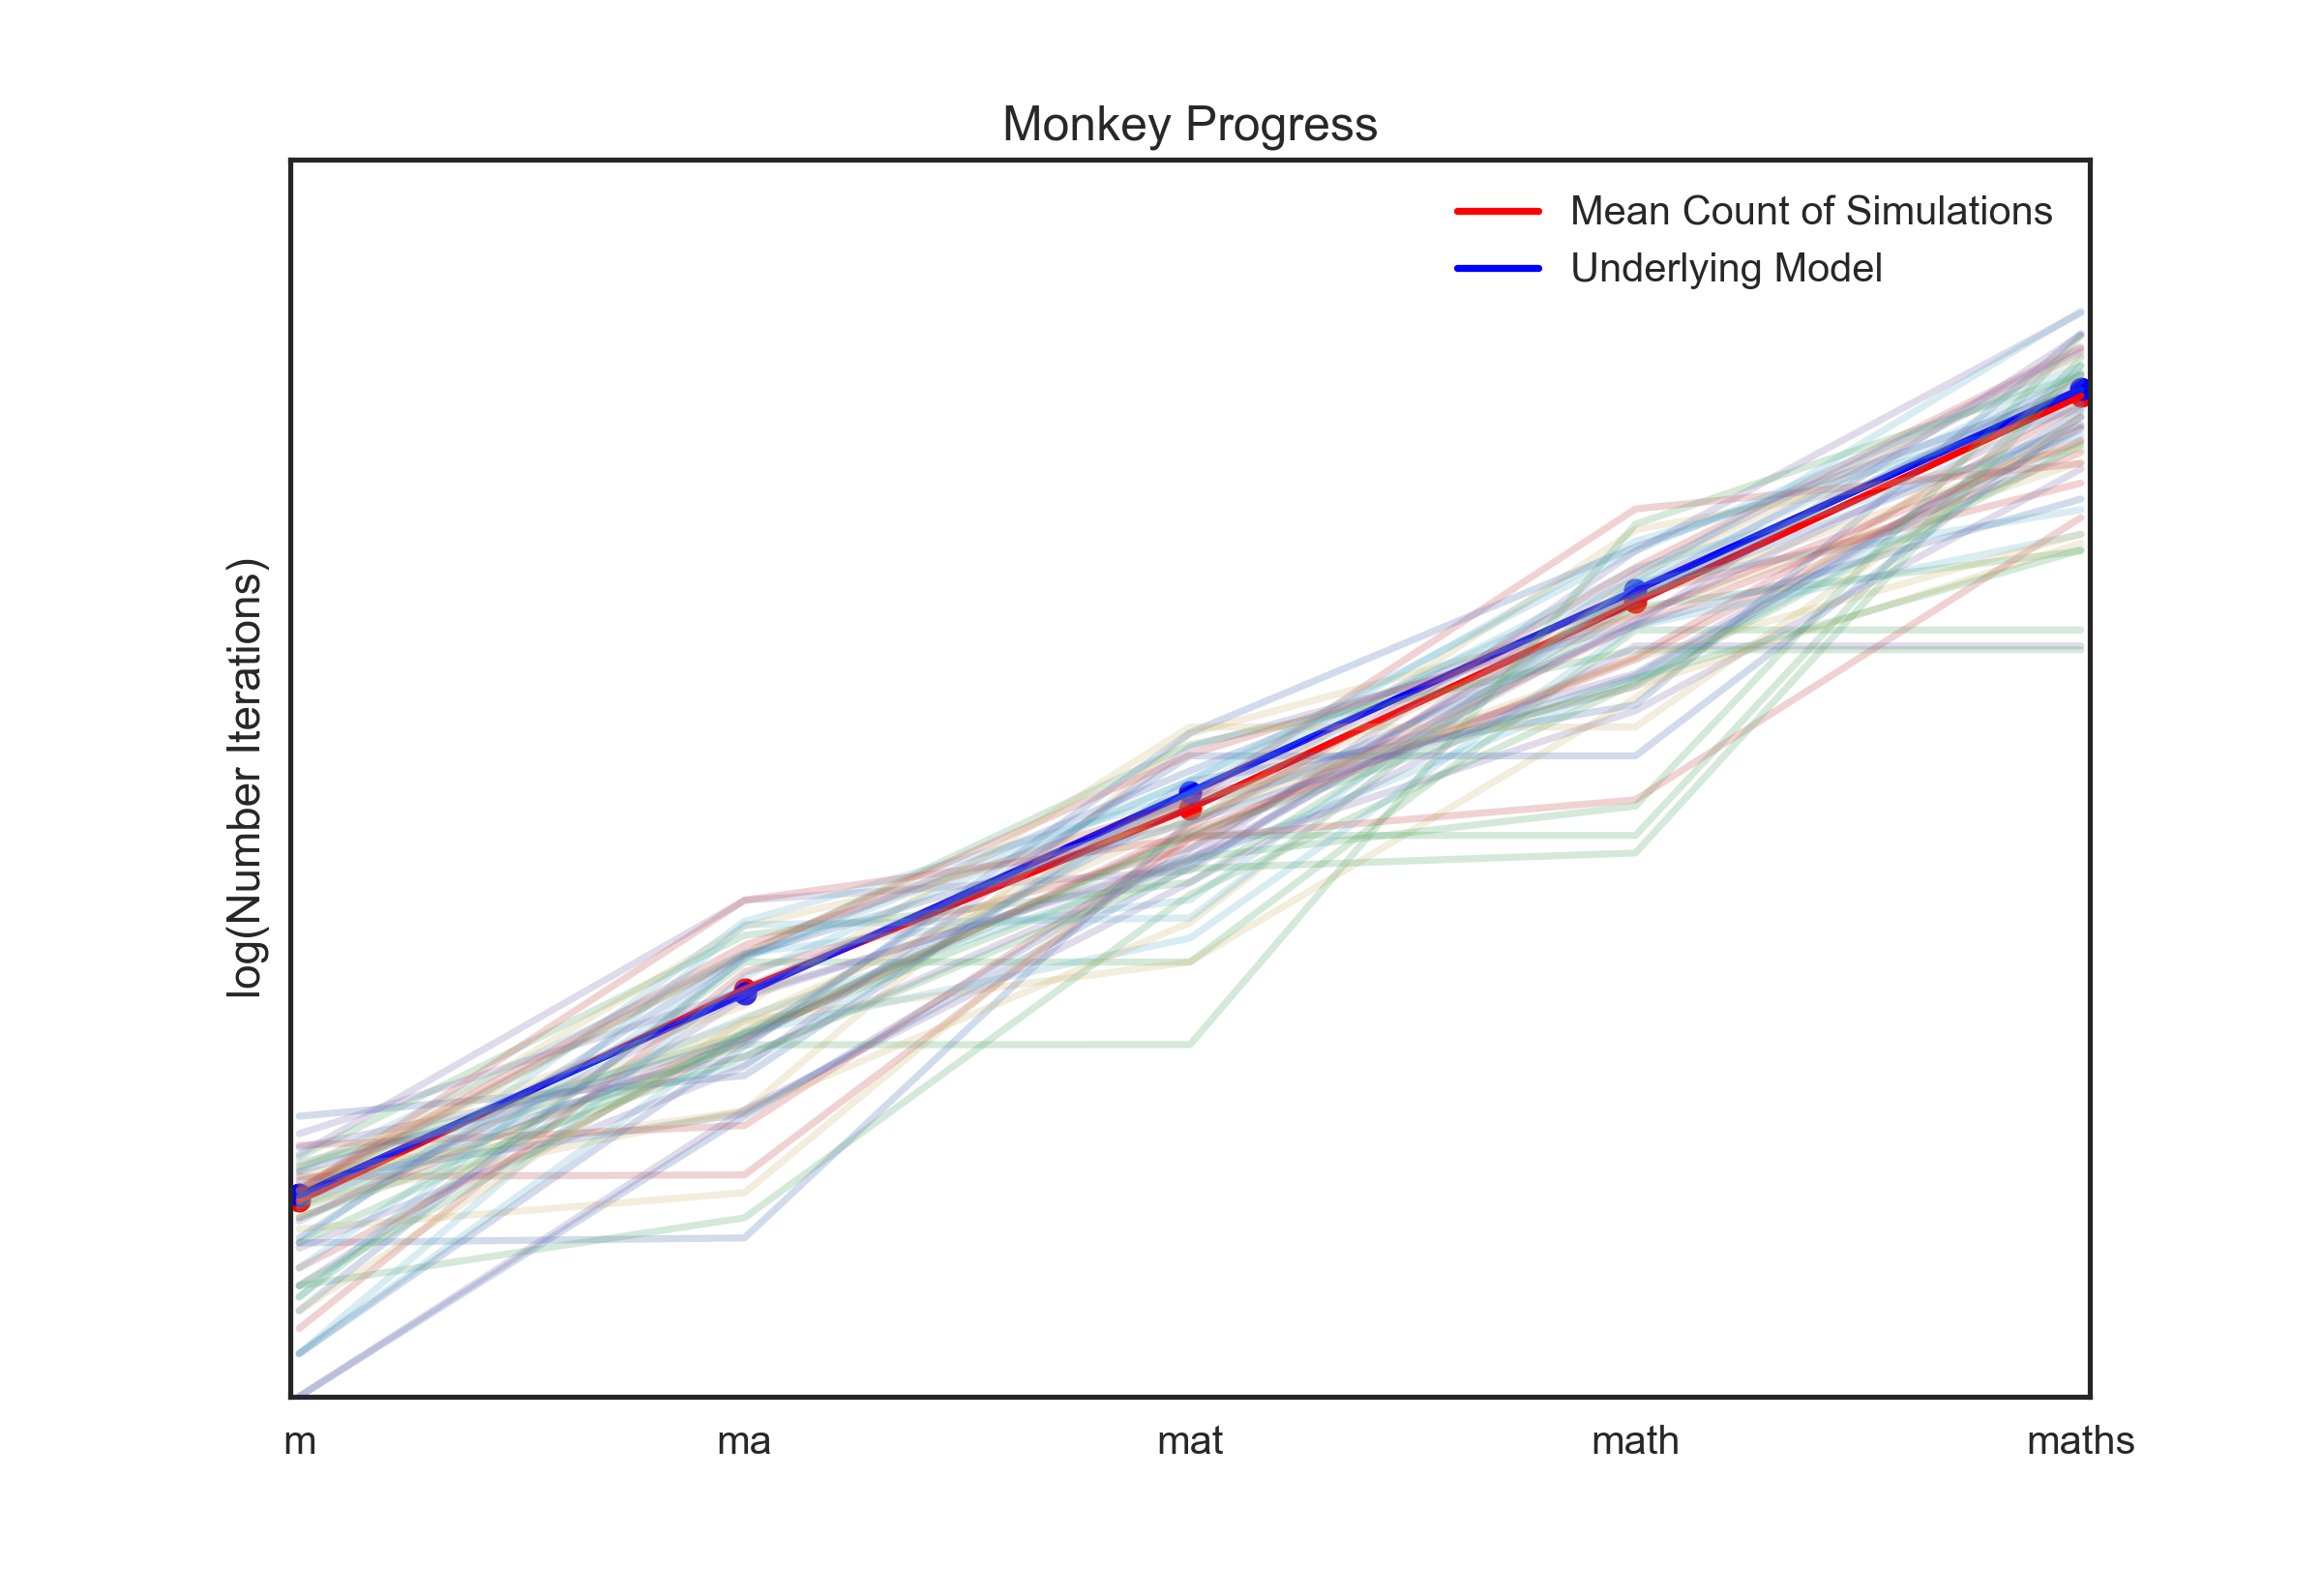
\includegraphics[width=0.90\textwidth]{log_approx}
    \caption{Logarithmic transformation}
\end{figure}


As expected, the number of keystrokes required to reach the next word increases at a really high rate. Despite this fact, since the model is a finite Markov chain we know there exists at least one recurrent state. Furthermore, this particular chain is in comunication with every other state. i.e. $$i \longleftrightarrow j \ \forall \ i,j \in S$$

Therefore this chain is recurrent.\\

Originally, this problem was set to answer whether our magical monkey could rewrite all Shakespeare's original plays. Mathematically, the answer is yes, and the monkey will do so an infinite number of times with probability 1! This is a consecuence of a recurrent chain.\\

As a quick back of the envelope calculation we can compute the number of keystrokes required to randomly wiriting all of Shakespeare's works. According to \texttt{opensourceshakespeare.org}, there are 884,421 words in Shakespeare's 43 works. If consider the english language at an average of 5 letter per word, that would make Shakespear's works 4,422,105 letters long, not including spaces or any sort of punctuation. Consecuently, it would take the monkey $26 ^ {4422105} $ keystrokes on average to complete the task.

\section{Conclusions}
Still a fun and interesting way to ponder about the implications of this markov chain, to me it is a clear evidence of the limitations of math under real-world constraints. On the one hand, we have a theorem that states that with probability one, this monkey will complete the task; on the other hand, we have an expected number of keystrokes so big that I could not even finished scrolling down (said number can be found at the bottom of \href{https://github.com/gerdm/UMA/blob/master/stochastic_processes/final_proyect/monkey_notebook.ipynb}{this page}).\\

Regardless, with the right considerations, a Markov chain is a powerful tool to model everyday behaviour. Certainly, I will be long gone by the time my Monkey finishes half my essay.

\newpage
\section{Appendix: Code}

\begin{Verbatim}[fontsize=\footnotesize]
import numpy as np
from numpy.random import choice
from collections import OrderedDict
import pickle

alphabet = "A B C D E F G H I J K L M N O P Q R S T U V W X Y Z".lower().split()
# The desired stream of words to be written
target_stream = "maths"

data_dict = OrderedDict()

# Iterate 50 instances of the monkey
for n_try in range(50):

    current_streak = ""
    streak_count = 0
    streaks_milestone = OrderedDict()
    count = 0
    max_streak = ""

    print("---------------------{}---------------------".format(n_try))
    while True:
        count += 1
        # Draw a single uniform sample from the alphabet
        sample_character = choice(alphabet)
        # If the sample character is the next caracter to write
        if sample_character == target_stream[streak_count]:
            streak_count += 1
            current_streak += sample_character

            # If a new streak is broken, save streak and iteration number
            if len(current_streak) > len(max_streak):
                streaks_milestone[current_streak] = count
                max_streak = current_streak

            # Print current state of simulation
            print(max_streak, count, end="\r")

        # If it misses, start over 
        else:
            streak_count = 0
            current_streak = ""

        if len(current_streak) == len(target_stream):
            break

    print(streaks_milestone)

    # Save current data to data_dict
    data_dict["round_" + str(n_try)] = streaks_milestone

# Pickle it
with open("monkey.pickle", "wb") as f:
    pickle.dump(data_dict, f)
\end{Verbatim}

\end{document}
